%%Berichtvorlage für EDBV WS 2014/2015

\documentclass[paper=A4, deutsch]{scrartcl}
\usepackage[ngerman]{babel}
\usepackage[utf8]{inputenc}
\usepackage{algorithmic}
\usepackage{algorithm}
\usepackage{graphicx}
\usepackage{amsmath,amssymb}
\usepackage{subcaption}
\captionsetup{compatibility=false}
\usepackage{multirow}
\usepackage{color}
\usepackage[]{geometry}
\graphicspath{ {./images/} }
\begin{document}


%%------------------------------------------------------
%% Ab hier tragt ihr eure Daten und Ergebnisse ein:
%%------------------------------------------------------

\title{nine-mans-morris} %%Projekttitel hier eintragen

\subtitle{EDBV WS 2018/2019: AG\_C3} %%statt XX Arbeitsgruppenbezeichnung hier eintragen (zB.: A1)


%%Namen und Matrikelnummern der Gruppenmitglieder hier eintragen
\author{Tobias Batik (11701221)\\
Bougouma Fall (01427956)\\
Yannic Ellhotka (11776168)\\
Simon Wesp (XXXXXXX)
}



%%------------------------------------------------------

\maketitle


%%------------------------------------------------------
\section{Gewählte Problemstellung}
(1-1,5 Seiten)\\
entspricht dem (aktualisierten) Konzept
\subsection{Ziel}
Ziel des Projekts\\
Brettspiel Muehle einlesen und moglichen naechsten Zug vorhersagen.
\subsection{Eingabe}
Folge von Farbbildern des Spielbrettes. 

\subsection{Ausgabe}
TODO müssen wir neu schreiben !!!!
\subsection{Voraussetzungen und Bedingungen}
Bilder muessen annaehernd in Volgelperspektive aufgenommen werden (+-30 Grad). \\
Das Spielbrett muss die in der Grafik dargestellten relativen Maßeinheiten erfüllen (siehe Abbildung 1) . 
Der Hintergrund der Spielfelder muss ausreichend Kontrast zu den weißen sowie schwarzen Spielsteinen aufweisen. \\
Die verwendeten Spielsteine haben eine durchmesser von Breite des Spielfelder * 0.08\\
Steine muessen eindeutig auf den vorgesehen Punkten liegen.\\

\begin{figure}[ht]
	\centering
		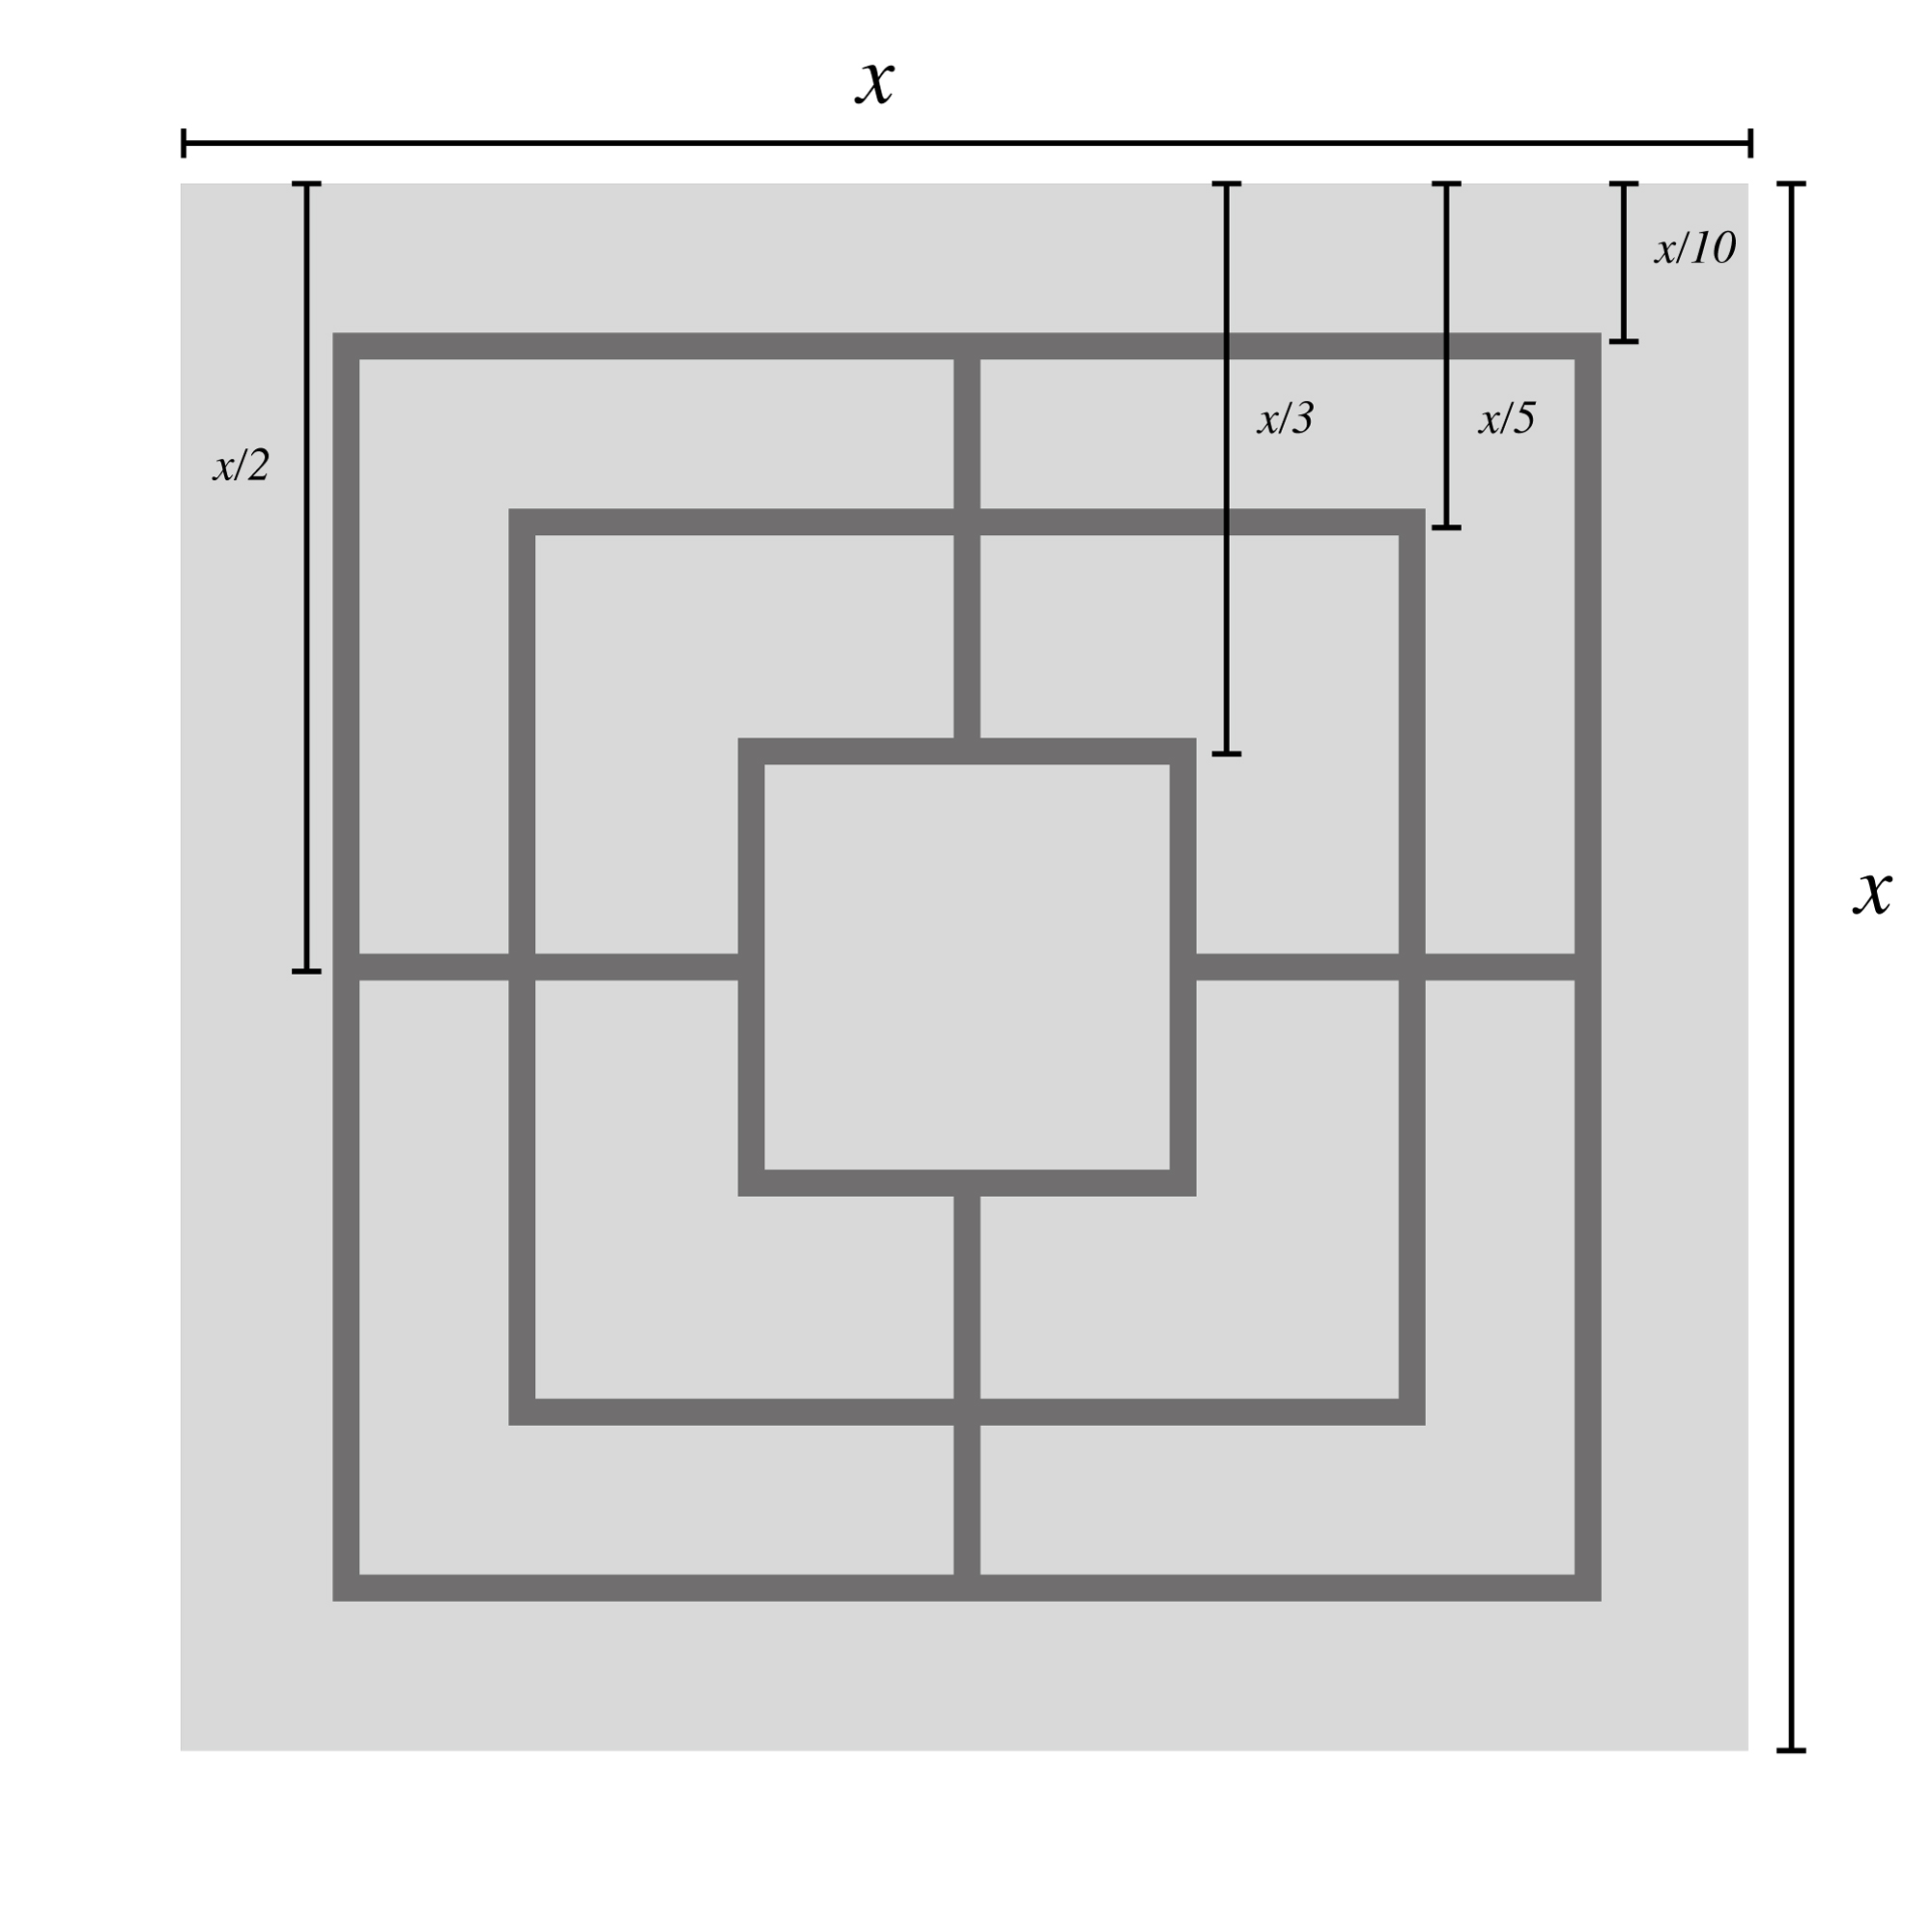
\includegraphics[width=8cm]{Spielbrett_relativeDimensionen_grafik.jpg}\\
	\caption[Relative Spielfelddimensionen]{Relative Spielfelddimensionen.}
	\label{fig:nettop}
\end{figure}



\subsection{Methodik}
1. Grauwert\\
\hspace*{1em} a. Input: RGB-Bild\\
\hspace*{1em} 	b. Output: Grauwertbild \\
2.  Threshold\\
\hspace*{1em} a. Input: Grauwertbild\\
\hspace*{1em} b. Output: Binärbild ???????? \\
3. Geometrische Transformation\\
\hspace*{1em} a. Input: Kantenbild und Koordinaten der Vierecke\\
\hspace*{1em} b. Output: transformiertes Kanten-Bild des Spielfeldes \\
4. Canny\\
\hspace*{1em} a. Input: Grauwertbild\\
\hspace*{1em} b. Output: Kantenbild \\
5. Hough-Transformation \\
\hspace*{1em} a. Input: transformiertes Kanten-Bild des Spielfeldes\\
\hspace*{1em} b. Output: Mittelpunkte der Spielsteine \\
6. Muss ich mir noch überlegen wie das heißt  \\
\hspace*{1em} a. Input: Mittelpunkte der Spielsteine und entzerrtes Graustufenbild\\
\hspace*{1em} b. Output: 3x3x3 Array das den aktuellen Spielstand repräsentiert \\
7. Algorithmus Zug berechnen Stimmt nicht mehr\\
\hspace*{1em} a. Input: Array des aktuellen Spielstands \\
\hspace*{1em} b. Output: Vorgeschlagener naaechster Zug

\subsection{Evaluierungsfragen}
1. Wird das Spielfeld richtig eingelesen?\\
2. Wird ein gueltiger Spielzug vorhergesagt?\\
\subsection{Zeitplan}
Der Zeitplan soll neben Euren anfänglichen, geplanten Zeiten/Arbeitsaufwände die tatsächlichen Zeiten/Arbeitsaufwände beinhalten. 
\begin{table}[h!]
	\centering
	\begin{tabular}{|c|c|c|c|c|}
		\hline
		Meilenstein & \multicolumn{2}{c|}{abgeschlossen am} & \multicolumn{2}{c|}{Arbeitsaufwand in h}\\
		\cline{2-5}
		 & geplant & tatsächlich & geplant & tatsächlich\\
		\hline
		...&... &... &... &...\\
		\hline
	\end{tabular}
\end{table}
%%------------------------------------------------------

%%------------------------------------------------------
\section{Arbeitsteilung}
(0,5 Seiten)\\
Wer hat welche Aufgaben übernommen (MATLAB-Funktionen, Abschnitt im Bericht, Evaluierung, Datenerfassung, etc.)? Die Aufteilung sollte fair sein, aber den tatsächlichen Aufwänden der einzelnen Teilnehmer entsprechen. Jeder übernimmt die Verantwortung (z.B. Korrektheit, keine Plagiate, wissen warum die Methode gewählt wurde) über seine ausgewiesenen Tätigkeiten.

\begin{center}
  \begin{tabular}{ |l | c | }
    \hline
  Name & Tätigkeiten\\
    \hline
		Vorname1 Nachname1 & Matlab-Funktion A, Bericht Abschnitt B...\\
		\hline
		Vorname2 Nachname2 & Matlab-Funktion C, Bericht Abschnitt D...\\
		\hline
		$\vdots$ & $\vdots$\\
  \end{tabular}
\end{center}

%%------------------------------------------------------

%%------------------------------------------------------
\section{Methodik}
(2-3 Seiten)\\
Hier wird die verwendete Methodik in der Theorie vorgestellt:\\
Welche Methodik wurde verwendet? Warum eignet sich diese Methodik für die gewählte Problemstellung? Habt ihr Methoden verändert (Einschränkungen, Abwandlungen, Parameter), wenn ja wie? etc.\\
Die erwähnten Methoden werden zum größten Teil auf Beschreibungen in Büchern oder wissenschaftlichen Artikeln beruhen. Daher ist hier auch der richtige Platz für Zitate. Die hier zitierten Publikationen sollten mittels Abkürzung bzw. Nummer referenziert sein und sich in der Referenzliste am Ende des Berichts über diese Bezeichnung finden lassen.\\
Ein Beispielsatz (inkl. entsprechender Literaturangabe am Ende des Berichts): Interest Points wurden mittels Scale Invariant Feature Transform \cite{lowe2004} detektiert.\\
Bei der Verwendung von Latex gestaltet sich das Zitieren besonders einfach - siehe Beispielssatz im Source der Latex-Vorlage.\\
\textbf{Wichtig in diesem Abschnitt ist, dass sich der Leser Eures Berichts mit den verwendeten Methodiken auskennt und weiß, weshalb ihr diese Methodiken verwendet habt und keine anderen. Es soll dem Leser helfen den nächsten Abschnitt des Berichts besser zu verstehen.}
%%------------------------------------------------------

%%------------------------------------------------------
\section{Implementierung}
(1-X Seiten)\\
Hier gebt ihr einen Überblick über Eure Implementierung:\\
Wie habt ihr die im vorhergehenden Abschnitt vorgestellte Methodik praktisch umgesetzt? Wie werden die einzelnen Methoden kombiniert (zB. Implementierungspipeline)?\\
Hier ist Platz für Implementierungsdetails wie zB. gewählte Parameter. \\
Wie startet der User das Programm? Welche Parameter hat der User zu setzen?\\
Auch in diesem Abschnitt können Referenzen und Zitate notwendig sein.\\
\textbf{Wichtig in diesem Abschnitt ist, dass der Leser Eures Berichts versteht wie ihr Euer Projekt in MATLAB umgesetzt habt um sich auch im Quelltext leichter zurechtfinden zu können.}
%%------------------------------------------------------

%%------------------------------------------------------
\section{Evaluierung}
(2-X Seiten)\\
Hier stellt ihr Euren Datensatz vor und beantwortet Evaluierungsfragen:\\
z.B. Fakten zum Datensatz: Anzahl der Bilder, Größe der Bilder, Quelle des Datensatzes (falls selbst aufgenommen: Aufnahmegerät, Einstellungen,... / falls nicht selbst erstellt: Datenbank vorstellen... $\to$ Referenzen!)\\
Diskussion der Evaluierungsfragen: Beantwortung der Fragen, Diskussion anhand von Beispielen, Diskussion von Grenzfällen: für welche Bilder funktioniert die Implementierung, für welche nicht? Worin unterscheiden sich diese Bilder? Warum funktionieren sie nicht? etc.\\
Evaluiert wird der ganze Datensatz, nicht nur einzelne Bilder. Einzelne Bilder können zum Aufzeigen von Fehlern/Problemen/besonders guten Ergebnissen... genutzt werden.\\
Zur Evaluierung gehört auch das Testen der einzelnen Methodiken (separat), mit Erwähnung eventueller Einschränkungen.
%%------------------------------------------------------

%%------------------------------------------------------
\section{Schlusswort}
(max. 1 Seite)\\
Hier fasst ihr Ergebnisse Eures Projekt zusammen:\\
Welche Schlussfolgerung lässt sich ziehen? Gibt es offene Probleme? Wie lässt sich Eure Lösung noch verbessern? etc.
%%------------------------------------------------------


%%------------------------------------------------------
\bibliographystyle{plain}
\bibliography{edbv_lit}
%%Bei verwendung von Latex schreibt ihr eure Referenzen in ein eigenes bib-File (siehe hier edbv_lit.bib). Jene Referenzen, die ihr im Bericht mittels \cite zitiert, werden automatisch in die Referenzliste übernommen. Weitere Information zum Einbinden von BibTex gibt es hier: http://www.bibtex.org/Using/de/
%%------------------------------------------------------
\textbf{Webseiten werden als Fußzeilen (an jener Stelle wo sie verwendet werden) eingebunden, nicht als Literature!}

\end{document}
\grid
\grid
